\documentclass[11pt,a4paper]{article} % Prepara un documento con un font grande

\usepackage{iftex}

\ifLuaTeX
  % Adatta LaTeX alle convenzioni tipografiche italiane,
% e ridefinisce alcuni titoli in italiano, come "Capitolo" al posto di "Chapter",
% se il documento è in italiano
%\usepackage[italian]{babel}
%\usepackage[utf8]{inputenc} % Consente l'uso caratteri accentati italiani
%\usepackage{graphicx}		% Per le immagini
%\usepackage{gnuplot-lua-tikz}
%\usepackage[top=2.5cm, bottom=2cm, left=2cm, right=2cm]{geometry}

%\nonstopmode %non fermarti agli errori

%\usepackage{fancyhdr}
%\setlength{\headheight}{15.2pt}
%\pagestyle{fancy} % Solo le pagine normali, non i titoli nè la pagina iniziale


%%%%%%%%%%%%%%%%%%%%%%%%%%%%%%%%%%%%%%%%%%%%%%%%%%%%%%%%%%%%%%%%%%%%%%%%%%%%%%%%%%%%%%%%%

\usepackage{lipsum} % Package to generate dummy text throughout this template

\usepackage{fontspec}
\setmainfont[Ligatures=TeX]{Alegreya}

%\usepackage[sc]{mathpazo} % Use the Palatino font
%\usepackage[T1]{fontenc} % Use 8-bit encoding that has 256 glyphs
%%%%%
%\usepackage{Alegreya} %% Option 'black' gives heavier bold face 
%\renewcommand*\oldstylenums[1]{{\AlegreyaOsF #1}}

%\usepackage[euler-digits,euler-hat-accent]{eulervm}
%%%%%%
%\usepackage[utf8]{inputenc} % Consente l'uso caratteri accentati italiani
%\linespread{1.05} % Line spacing - Palatino needs more space between lines
\usepackage{amsmath, amsthm, amssymb, amsfonts}
\usepackage{microtype} % Slightly tweak font spacing for aesthetics

%%%%%%%%%%%%%%%%%%%%%%%%%%%%%%%%%%%%%%%%%%%%%
%Miei package
\usepackage[italian]{babel}
\usepackage{graphicx}		% Per le immagini
\usepackage{gnuplot-lua-tikz}
%%%%%%%%%%%%%%%%%%%%%%%%%%%%%%%%%%%%%%%%%%%%%
\usepackage[hmarginratio=1:1,top=32mm,columnsep=20pt]{geometry} % Document margins
\usepackage{multicol} % Used for the two-column layout of the document
\usepackage[hang, small,labelfont=bf,up,textfont=it,up]{caption} % Custom captions under/above floats in tables or figures
\usepackage{booktabs} % Horizontal rules in tables
\usepackage{float} % Required for tables and figures in the multi-column environment - they need to be placed in specific locations with the [H] (e.g. \begin{table}[H])
\usepackage{hyperref} % For hyperlinks in the PDF

\usepackage{lettrine} % The lettrine is the first enlarged letter at the beginning of the text
\usepackage{paralist} % Used for the compactitem environment which makes bullet points with less space between them

\usepackage{abstract} % Allows abstract customization
\renewcommand{\abstractnamefont}{\normalfont\bfseries} % Set the "Abstract" text to bold
\renewcommand{\abstracttextfont}{\normalfont\small\itshape} % Set the abstract itself to small italic text

\usepackage{titlesec} % Allows customization of titles
\renewcommand\thesection{\Roman{section}} % Roman numerals for the sections
\renewcommand\thesubsection{\Roman{subsection}} % Roman numerals for subsections
\titleformat{\section}[block]{\large\scshape\centering}{\thesection.}{1em}{} % Change the look of the section titles
\titleformat{\subsection}[block]{\large}{\thesubsection.}{1em}{} % Change the look of the section titles

\usepackage{fancyhdr} % Headers and footers
\pagestyle{fancy} % All pages have headers and footers
\fancyhead{} % Blank out the default header
\fancyfoot{} % Blank out the default footer
\fancyhead[C]{Running title $\bullet$ November 2012 $\bullet$ Vol. XXI, No. 1} % Custom header text
\fancyfoot[RO,LE]{\thepage} % Custom footer text


\else
  % Adatta LaTeX alle convenzioni tipografiche italiane,
% e ridefinisce alcuni titoli in italiano, come "Capitolo" al posto di "Chapter",
% se il documento è in italiano
%\usepackage[italian]{babel}
%\usepackage[utf8]{inputenc} % Consente l'uso caratteri accentati italiani
%\usepackage{graphicx}		% Per le immagini
%\usepackage{gnuplot-lua-tikz}
%\usepackage[top=2.5cm, bottom=2cm, left=2cm, right=2cm]{geometry}

%\nonstopmode %non fermarti agli errori

%\usepackage{fancyhdr}
%\setlength{\headheight}{15.2pt}
%\pagestyle{fancy} % Solo le pagine normali, non i titoli nè la pagina iniziale


%%%%%%%%%%%%%%%%%%%%%%%%%%%%%%%%%%%%%%%%%%%%%%%%%%%%%%%%%%%%%%%%%%%%%%%%%%%%%%%%%%%%%%%%%

\usepackage{lipsum} % Package to generate dummy text throughout this template

%\usepackage[sc]{mathpazo} % Use the Palatino font
\usepackage{tgpagella} % TeX Gyre Pagella, versione migliorata di Palatino. Si ma bo, no
%\usepackage{inconsolata} % Font monospace
\usepackage{textcomp}
\usepackage[scale=0.98,ttdefault]{AnonymousPro}

%%%%%
%\usepackage{Alegreya} %% Option 'black' gives heavier bold face 
\usepackage{AlegreyaSans} %% Option 'black' gives heavier bold face 
%\renewcommand*\oldstylenums[1]{{\AlegreyaOsF #1}}
%\usepackage{opensans}
%\usepackage[euler-digits,euler-hat-accent]{eulervm}
\usepackage[euler-hat-accent]{eulervm}
%%%%%%

\usepackage[T1]{fontenc} % Use 8-bit encoding that has 256 glyphs

\usepackage[utf8]{inputenc} % Consente l'uso caratteri accentati italiani
\linespread{1.08} % Line spacing - Palatino needs more space between lines, messo a 1.08 da 1.11 che era per alegreya
\usepackage{amsmath, amsthm, amssymb, amsfonts}
\usepackage[italian]{babel}
%\usepackage[kerning,spacing,tracking,letterspace = 2,babel]{microtype} % Slightly tweak font spacing for aesthetics. Il tre è pensato per Alegreya
\usepackage[kerning,spacing,babel]{microtype}
\SetTracking[]{encoding = *,shape = *}{3} % Aumenta la distanza fra le lettere
							     % http://tex.stackexchange.com/questions/66494/new-command-for-spacing-letters-in-microtype
%%%%%%%%%%%%%%%%%%%%%%%%%%%%%%%%%%%%%%%%%%%%%
%Miei package



\usepackage{graphicx}		% Per le immagini
\usepackage{fixltx2e}
%\usepackage{color}		% COLORI!

%\definecolor{grigio-molto-scuro}{gray}{0.1}	%colore

\usepackage{tabularx}		% Per le tabelle con le colonne tutte uguali
\usepackage{tabulary}		% Tabelle migliorate, nelle celle il testo va a capo da solo...
\usepackage{gnuplot-lua-tikz}
%%%%%%%%%%%%%%%%%%%%%%%%%%%%%%%%%%%%%%%%%%%%%
\newlength{\alphabet}
\settowidth{\alphabet}{\normalfont abcdefghijklmnopqrstuvwxyz}
\usepackage[
	    %hmargin=0.18\paperwidth,% metti la larghezza del testo (margini orizzontali) al 18% del foglio
	    textwidth=2.4\alphabet,  % http://tex.stackexchange.com/questions/59626/nicely-force-66-characters-per-line
	    hmarginratio=1:1,       % margini destro e sinistro uguali
	    top=35mm,	            % margine sopra a 32mm...
	    vmarginratio=4:5,       % quello sotto uguale (default 2:3)
	    columnsep=20pt]         % Spazio tra le colonne?
	    {geometry} % Document margins
\usepackage{multicol} % Used for the two-column layout of the document
\usepackage[hang, small,labelfont=bf,up,textfont=it,up]{caption} % Custom captions under/above floats in tables or figures
\usepackage{booktabs} % Horizontal rules in tables
\usepackage{float} % Required for tables and figures in the multi-column environment - they need to be placed in specific locations with the [H] (e.g. \begin{table}[H])
%\usepackage{tocloft} % Per customizzare le liste di floats (per i custom float!)
\usepackage[titles]{tocloft} %Pare causi meno casini con fancyhdr
\usepackage{nicefrac} % Per le frazioni tipo ⅛
\usepackage{pdfpages} % Per includere pagine intere in pdf (per la copertina)
%\usepackage[squaren]{siunitx}

\usepackage{lettrine} % The lettrine is the first enlarged letter at the beginning of the text
\usepackage{paralist} % Used for the compactitem environment which makes bullet points with less space between them
\usepackage[section]{placeins} % Per \FloatBarrier. L'opzione section comporta che le sezioni siano floatbarriers

\usepackage{abstract} % Allows abstract customization
\renewcommand{\abstractnamefont}{\normalfont\bfseries} % Set the "Abstract" text to bold
\renewcommand{\abstracttextfont}{\normalfont\small\itshape} % Set the abstract itself to small italic text

\usepackage{caption} % Per captions avanzate

\usepackage{listingsutf8} % Per includere codice sorgente meglio che con verbatim (e con caratteri non inglesi)
\lstset{ 
  %Preso anche questo da http://en.wikibooks.org/wiki/LaTeX/Source_Code_Listings
  %backgroundcolor=\color{white},   % choose the background color; you must add \usepackage{color} or \usepackage{xcolor}
  basicstyle=\footnotesize\ttfamily,        % the size of the fonts that are used for the code E MESSO IN MONOSPACE
  breakatwhitespace=true,         % sets if automatic breaks should only happen at whitespace
  breaklines=true,                 % sets automatic line breaking
  captionpos=b,                    % sets the caption-position to bottom
  %commentstyle=\color{mygreen},    % comment style
  %deletekeywords={...},            % if you want to delete keywords from the given language
  %escapeinside={\%*}{*)},          % if you want to add LaTeX within your code
  %extendedchars=true,              % lets you use non-ASCII characters; for 8-bits encodings only, does not work with UTF-8
  frame=l,                    % adds a frame around the code
				    %you can control the rules at the top, right, bottom, and left directly by using the four initial 
				    %letters for single rules and their upper case versions for double rules. http://mirror.hmc.edu/ctan/macros/latex/contrib/listings/listings.pdf
				    % Es frame frame=trBL ha doppia linea a sinistra e sotto, e singola a destra e sopra
  keepspaces=true,                 % keeps spaces in text, useful for keeping indentation of code (possibly needs columns=flexible)
  %keywordstyle=\color{blue},       % keyword style
  %language=Octave,                 % the language of the code
  %morekeywords={*,...},            % if you want to add more keywords to the set
  numbers=left,                    % where to put the line-numbers; possible values are (none, left, right)
  numbersep=5pt,                   % how far the line-numbers are from the code
  %numberstyle=\tiny\color{mygray}, % the style that is used for the line-numbers
  %rulecolor=\color{black},         % if not set, the frame-color may be changed on line-breaks within not-black text (e.g. comments (green here))
  showspaces=false,                % show spaces everywhere adding particular underscores; it overrides 'showstringspaces'
  showstringspaces=false,          % underline spaces within strings only
  showtabs=false,                  % show tabs within strings adding particular underscores
  stepnumber=1,                    % the step between two line-numbers. If it's 1, each line will be numbered
  %stringstyle=\color{mymauve},     % string literal style
  tabsize=2,                       % sets default tabsize to 2 spaces
  title=\lstname                   % show the filename of files included with \lstinputlisting; also try caption instead of title
}


\usepackage{titlesec} % Allows customization of titles
\renewcommand\thesection{\Roman{section}} % Roman numerals for the sections
\renewcommand\thesubsection{\Roman{subsection}} % Roman numerals for subsections
% \usefont {encoding} {family} {series} {shape}
\titleformat{\section}[block]{\AlegreyaSansSC \bfseries \LARGE}{\thesection.}{1em}{} % Change the look of the section titles. Pezzi spostati \scshape\centering\bfseries
\titleformat{\subsection}[block]{\AlegreyaSans \bfseries \Large}{\thesection.\thesubsection }{1em}{} % Change the look of the section titles

\usepackage{fancyhdr} % Headers and footers
\pagestyle{fancy} % All pages have headers and footers
\fancyhead{} % Blank out the default header
\fancyfoot{} % Blank out the default footer
\headheight=14pt % Perchè sennò continua a lamentarsi che 12pt è troppo poco e la mette a 14 lo stesso
%\fancyhead[C]{Chiappara, Labanca, Forcher - \textit{Ottica geometrica} $\bullet$ \thesection}
\fancyhead[L]{\textit{Ottica geometrica}} % Custom header text. \nouppercase{\leftmark} per sezione, ma non ci sta
\fancyhead[R]{\textsc{\nouppercase{\leftmark}}}
\fancyfoot[RO,LE]{\thepage} % Custom footer text

\usepackage[hidelinks]{hyperref} % For hyperlinks in the PDF
\hypersetup{
    bookmarks=true,         % show bookmarks bar?
    unicode=false,          % non-Latin characters in Acrobat’s bookmarks
   % pdftoolbar=true,        % show Acrobat’s toolbar?
   % pdfmenubar=true,        % show Acrobat’s menu?
   % pdffitwindow=false,     % window fit to page when opened
    %pdfstartview={FitH},    % fits the width of the page to the window
    pdftitle={Ottica geometrica},    % title
    pdfauthor={D. Chiappara, G. Labanca, F. Forcher},     % author
    pdfsubject={Relazione di ottica geometrica - Sperimentazioni II 2014},   % subject of the document
    %pdfcreator={Creator},   % creator of the document
    %pdfproducer={Producer}, % producer of the document
    pdfkeywords={ottica} {geometrica} {relazione} {Sperimentazioni}, % list of keywords
    %pdfnewwindow=true,      % links in new PDF window
    %colorlinks=false,       % false: boxed links; true: colored links
    linkcolor=red,          % color of internal links (change box color with linkbordercolor)
    citecolor=green,        % color of links to bibliography
    filecolor=magenta,      % color of file links
    urlcolor=cyan           % color of external links
}

\fi
\DeclareGraphicsExtensions{.pdf, .png, .jpg} % Se due immagini hanno lo stesso nome sceglile secondo l'ordine di filetype qui
\graphicspath{ {./img/} }					 % Path delle immagini 

\title{
\vspace{-2cm}
\fontsize{48pt}{10pt}\selectfont
\textsc{Relazione di \\[3mm] Elettronica}
}
% \title{}
\author{
\large
\textsc{Francesco Forcher}\\[2mm]
\normalsize Università di Padova, Facoltà di Fisica\\
\normalsize francesco.forcher@studenti.unipd.it\\
\normalsize Matricola: \texttt{1073458}\\
\and
\large
\textsc{Davide Chiappara}\\[2mm]
\normalsize Università di Padova, Facoltà di Fisica\\
\normalsize davide.chiappara@studenti.unipd.it\\
\normalsize Matricola: \texttt{1070160}\\
\and
\large
\textsc{Gabriele Labanca}\\[2mm]
\normalsize Università di Padova, Facoltà di Fisica\\
\normalsize gabriele.labanca@studenti.unipd.it\\
\normalsize Matricola: \texttt{1069556}
}
\date{\today}

%%%%%%%%%%%%%%%%%%%%%%%%%%%%%%%%%%%%%%5%%%%%%%%%%%%%%%%%%%%%%%%%%%%%%%%%%%%%%%%%%%
%\usepackage{float}
%\usepackage{caption}
%\usepackage{multirow}
%\usepackage[top=3.6cm, bottom=1.5in, left=0.5in, right=0.5in]{geometry}

%%%%%%%%%%%%%%%%%
% Robe del package tocloft per fare gli indici delle mie tabelle e grafici
% texblog.org/2008/07/13/define-your-own-list-of/
%\newcommand{\listtabellaname}{Lista delle tabelle}
%\newlistof{tabella}{tab}{\listtabellaname}


%%%%%%%%%%%%%%%%%

% I miei stili di float, con le righe
\floatstyle{plaintop}
\newfloat{tabella}{tb}{lop} 
\floatname{tabella}{Tabella}

\floatstyle{ruled}
\newfloat{grafico}{tb}{loi} 
\floatname{grafico}{Grafico}

\newcommand{\tabellaautorefname}{\bfseries Tabella} % per \autoref del package hyperref
\newcommand{\graficoautorefname}{\bfseries Grafico} % Idem



%%%%%%%%%%%%%%%%%%%%%%%%%%%%%%%%%%%%%%%%%%%%%%%%%%%%%%%%%%%%%%%%%%%%%5%%%%%%%%%%%%%
% Comandi personalizzati

% \newcommand{\cm}{\,\mathrm{cm}}
% \DeclareMathOperator{\cov}{cov} % Covarianza
% \DeclareMathOperator{\var}{var} % Covarianza
% \newcommand{\mm}{\,\mathrm{mm}}
% \newcommand{\nm}{\,\mathrm{nm}}
% \newcommand{\usuq}{\nicefrac{1}{q}}
% \newcommand{\usup}{\nicefrac{1}{p}}



%////////////////////////////////////////////////////////////////////////////////////////////////////////////////////////////
%////////////////////////////////////////////////////////////////////////////////////////////////////////////////////////////
% Fine dei dati iniziali per il latex: il documento finale inizierà da qui
\begin{document}

%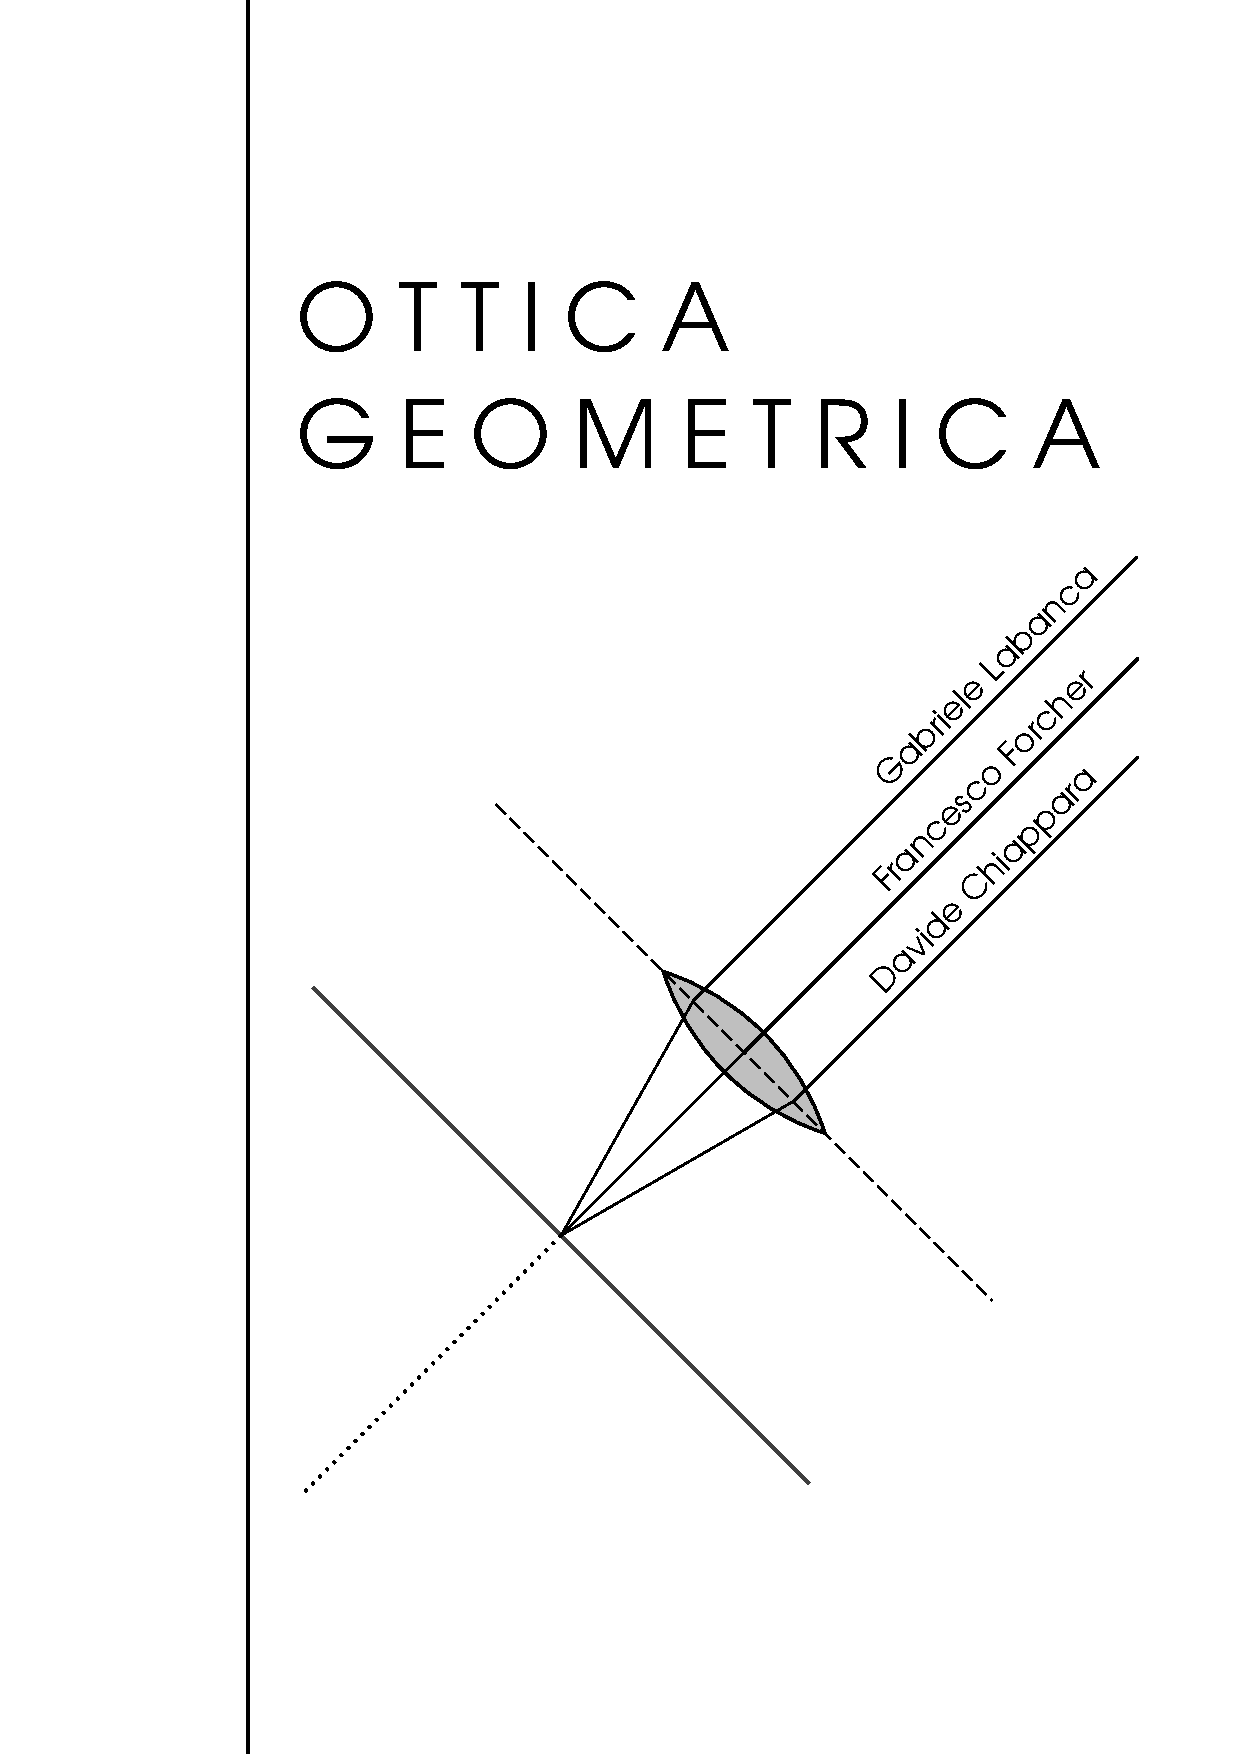
\includepdf[pages={1}]{./img/copertina_relazione.pdf}

{
%\color{grigio-molto-scuro}
%\lsstyle % Abilita il letterspacing personalizzato
%\unclfamily % Cagata per il font Uncial

\maketitle % Produce il titolo a partire dai comandi \title, \author e \date

\vspace{ \stretch{1} }
\begin{center}
	%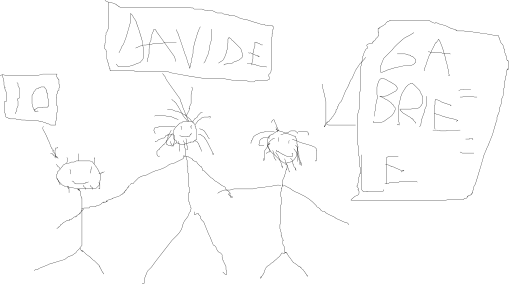
\includegraphics[width=0.7\textwidth]{gruppo_rel}
\end{center}

\vspace{ \stretch{1} }
% Le varie sezioni
%\section{Obiettivi}
\begin{abstract}
	\noindent
	Sono stati costruiti dei circuiti elementari e sono state misurate le
resistenze interne degli strumenti di misura. Si è inoltre verificata
la validità della legge di Ohm.
\end{abstract}

\newpage


\microtypesetup{protrusion=false} % disables protrusion locally in the document
\tableofcontents % prints Table of Contents
%\listoftabella
%\listoffigures
%\listoftables
\microtypesetup{protrusion=true} % enables protrusion

%\begin{multicols}{2}

% \section{Apparato strumentale}
% 	Strumentazione utilizzata (banco ottico numero 5):
\begin{itemize}
\item Guida ottica di lunghezza $\approx 140 \cm$ con scala graduata con passo 0.5 mm;
\item Generatore di corrente di intensità e voltaggio regolabili;
\item Lampada;
\item Cavaliere portalampada con tre filtri cromatici e un portamascherine;
\item Cavaliere portalente con micrometro (valore di azzeramento $8.60 \mm$);
\item Cavaliere portalente senza micrometro;
\item Cavaliere portaschermo con due micrometri;
\item Cavaliere portasquadra;
\item Mascherina con buco centrale;
\item Diaframma con singolo buco centrale;
\item Diaframma con 2 buchi marginali e 2 parassiali posti su segmenti ortogonali;
\item Lente numero 3;
\item Doppietto di Dollond;
\item Oculare con ingrandimento di 8x.
\end{itemize}


% \section{Metodologia di misura}
% 	L'esperienza \`e suddivisa in 5 fasi diverse, ognuna con un'approccio sperimentale e un'analisi dati differente. Questa sezione ha lo scopo di descrivere la metodologia prescelta dagli sperimentatori in laboratorio, dunque non vi si discutono le scelte numeriche fatte o le analisi dati, un'accurata descrizione delle quali è fornita nelle sezioni successive.


Preliminarmente a ogni esperienza, è stato necessario preparare il banco ottico con la seguente procedura: in primo luogo tutti i micrometri sono portati allo zero della scala, dopodichè il cavaliere portalampada \`e fissato in un punto arbitrario della guida; tale punto è stato scelto il più marginalmente possibile sulla sinistra per avere spazio a disposizione per gli altri cavalieri. Bloccato con la vite il cavaliere portalampada, si utilizza il cavaliere con squadra per andare a leggere sulla scala millimetrata il valore che, dopo aver finito la preparazione dell'apparato sperimentale, corrisponder\`a alla posizione dell'oggetto relativa alla guida ottica. Il cavaliere con squadra va subito rimosso dalla guida ottica. Fatto ciò, viene montata la mascherina con foro singolo sull'apposito supporto presente sul cavaliere portalampada, mantenendo l'anello di fissaggio rivolto a destra. 

Sistemato il cavaliere portalampada, il cavaliere portalente viene posizionato sulla guida ottica e vi si avvita la lente sul lato destro, poi il diaframma sul sinistro. \'E necessaria particolare attenzione nell'avvitare la lente fino alla fine del filo delle componenti meccaniche del sistema. Alla sinistra del portalente non ancora fissato va posto il cavaliere portaschermo con micrometro, in modo tale che lo schermo sia rivolto verso sinistra, e si inserisce nel cavaliere portalampada il filtro di colore giallo.


Per stimare la lunghezza focale attraverso il metodo dell'autocollimazione si è operato spostando il cavaliere portalente con micrometro sulla guida ottica manuale o attraverso il micrometro, e tramite lettura di valori sul metro posto sulla guida o sui micrometri. Il diaframma utilizzato per questa esperienza è quello con un singolo foro centrale. 

Preparato il banco ottico, prima di iniziare la vera e propria presa dati si è cercato approssimativamente quale potesse essere la posizione del fuoco della lente. Si è quindi mosso il cavaliere portalente e successivamente confrontata grossolanamente la dimensione delle proiezioni del raggio sullo schermo quando esso veniva posto vicino o lontano dal cavaliere portalente. Eseguita una volta questa operazione, essa è stata ripetuta più volte muovendo il cavaliere portalente a sinistra o a destra a seconda che l'immagine nello schermo fosse più grande rispettivamente nel caso lo schermo fosse posto più vicino o più lontano dalla lente. Una reiterazione di queste azioni ha permesso dopo circa 4-5 ripetizioni di trovare un punto per il cavaliere portalente per il quale il cerchio proiettato sullo schermo fosse di grandezza approssimativamente costante al muoversi del cavaliere portaschermo. 

Trovato il punto, ci si è spostati a destra di circa mezzo centimetro (iniziando con il valore zero della scala del micrometro sono possibili infatti solo spostamenti dello stesso che avvicinano la lente alla lampada, non c'è modo di allontanarle) e si è saldamente bloccato il cavaliere portalampada con l'apposita vite. Il valore letto dall'indice del cavaliere portalente è stato registrato e poi è stata iniziata la vera e propria presa dati. Per prima cosa è stato regolato il micrometro in modo tale che la lente fosse spostata di circa mezzo centimetro, in modo cioè che si trovasse sul punto nel quale a occhio era stata individuata la condizione di fascio parallelo. Successivamente, si è misurato il diametro a posizioni costanti dello schermo (da vicino, $20\cm$; da lontano, $130\cm$).
Per fare ciò, è stato utilizzato il reticolo presente sullo schermo smerigliato: operando con il micrometro che permetteva allo schermo uno spostamento perpendicolare all'asse ottico, sono state misurate le posizioni che esso segnava quando una linea del reticolo diventava tangente al cerchio luminoso. Presi i dati, il diametro del cerchio \`e stato ottenuto sommando un centimetro alla differenza ottenuta, come risulta evidente dalla costruzione fisica del sistema. Confrontando i dati con la stessa logica dei passaggi precedenti, anche grazie a un programma che consentiva di visualizzarli istantaneamente su un grafico, si è spostata la lente avvicinandola o allontanandola dall'oggetto andando a operare sul micrometro presente nel cavaliere portalente. Trovato il punto in cui la differenza tra il diametro proiettato sullo schermo più distante e quello proiettato sullo schermo più prossimo cambiasse segno, si è indagato con maggiore precisione sull'area compresa tra le due misurazioni.


Per trovare il fuoco attraverso il metodo dei punti coniugati, il cavaliere portalampada \`e stato bloccato, ma, a differenza di quella precedente, non si è bloccato il cavaliere portalente. Si è operato senza micrometri, solamente spostando i cavalieri lungo la guida ottica, e come nell'esperienza precedente si è utilizzato il diaframma con singolo buco centrale. Preparato il banco ottico si è posto il cavaliere portalente inizialmente a una distanza dal cavaliere portalampada maggiore del fuoco che era stato stimato con il metodo dell'autocollimazione. Muovendo il cavaliere portaschermo si è cercato il punto in cui il raggio proiettato presentava diametro più piccolo possibile (per vederlo con più facilità si è fatto uso dell'oculare in dotazione), a quel punto si sono registrati su una tabella la posizione del cavaliere portalente e quella del cavaliere portaschermo. Il cavaliere portalente è stato poi spostato a destra e si è ripetuta l'operazione, aggiungendo una riga alla tabella precedentemente fatta. Il processo è stato ripetuto indagando il più uniformemente possibile le posizioni permesse dalla guida ottica.

Per trovare il fuoco attraverso il metodo di Bessel, sono stati tenuti fermi i cavalieri portalampada e quello portaschermo e si è mosso solamente il cavaliere portalente. Si è preparato il banco ottico e utilizzato il diaframma con buco singolo e il cavaliere portalente senza micrometro. Per prima cosa, data l'analisi teorica che si può fare a riguardo, si è bloccato il cavaliere protalampada il più a sinistra possibile (come nelle altre esperienze) e, utilizzando le stime fatte con le altre esperienze, si è bloccato il cavaliere portaschermo a più di $4f$. Muovendo il cavaliere portalente, si sono cercate le due posizioni per cui l'immagine andasse a fuoco. Nel caso non risultasse evidente distinguere un fuoco dall'altro si è allontanato ulteriormente il cavaliere portaschermo. Trovata una posizione dei due cavalieri fissi tale che i due fuochi fossero facilmente distinguibili e i cavalieri non fossero troppo lontani tra loro, si è iniziata la presa dati. Aiutandosi con l'oculare, è stata misurata la posizione della lente per la quale il fascio fosse a fuoco sullo schermo. Spostando il cavaliere portalente è stato, successivamente, registrato il punto in cui l'immagine fosse nuovamente a fuoco nonostante la diversa posizione. Tali misurazioni di posizione sono stati ripetute 10 volte ciascuna.


Per quanto riguarda la stima dell'aberrazione sferica caratterizzante la lente, si è preparato il banco ottico con i cavalieri portalenti: quello con micrometro montante il doppietto di Dollond e quello senza micrometro montante la lente. Inizialmente non è stato applicato alcun diaframma ed è stato posizionato sulla guida ottica solamente il cavaliere con il doppietto acromatico. Grazie ad una bacchettina lunga circa quanto la distanza focale del doppietto, si è bloccato il cavaliere portalente in una posizione tale che l'oggetto occupasse uno dei suoi fuochi. Per fare ciò si bloccata tale barretta sospendendola per attrito tra il doppietto e la mascherina montata sul cavaliere portalampada; a quel punto il cavaliere con il doppietto acromatico è stato bloccato con la vite. Successivamente, spingendo la lente verso sinistra mantenendo la vite del cavaliere portalente avvitata, grazie alla molla presente all'interno del micrometro, è stata rimossa la bacchettina. Analogamente a quanto fatto nel caso dell'autocollimazione (ma con il doppietto di Dollond e senza diaframma) è stato cercato velocemente il punto in cui il diametro della proiezione sullo schermo sembrava costante al variare della posizione del cavaliere portaschermo. Dopo aver aggiustato un paio di volte con il micrometro la posizione della lente, si è potuto utilizzare il raggio parallelo cos\`i creato per la misurazione dell'aberrazione sferica. Tra il cavaliere con il doppietto acromatico e il cavaliere portaschermo si \`e posto il cavaliere con lente, al quale è stato avvitato il diaframma con 4 buchi, in modo tale che i due buchi marginali fossero su un piano orizzontale. Il cavaliere portalente senza micrometro è stato posizionato il più vicino possibile all'altro cavaliere portalente, in modo che non ci fossero dispersioni del fascio uniforme legate alla distanza e che tutti e 4 i buchi del diaframma fossero ben illuminati. Fatto ciò, si è regolato il cavaliere portaschermo fino a trovare approssimativamente il punto in cui le 4 immagini si avvicinassero a formare quasi un punto unico. Si è bloccato il cavaliere portaschermo in quel punto e poi, operando sul micrometro, si è verificato che il movimento dello schermo permettesse di raggiungere agevolmente la posizione nella quale i 4 punti erano ancora separati e la posizione nella quale i 4 punti se separavano di nuovo nettamente. Fatto ciò è stato possibile iniziare la presa dati, per la quale è stato utilizzato solamente il micrometro che permetteva allo schermo uno spostamento parallelo all'asse ottico. Partendo dal punto per il quale i 4 punti erano ben distinti si è cercato il punto in cui i raggi marginali convergessero in un unico punto, facendo vedere l'immagine all'oculare come tre punti allineati verticalmente. Una volta registrato il valore letto sul micrometro, si è portato avanti il micrometro fino a vedere i tre punti allineati orizzontalmente. Questo valore è stato registrato e poi si è registrata la posizione nella quale sullo schermo fossero ancora visibili tre punti orizzontali. Questi ultimi due valori sono stati presi in modo che i punti si vedessero allineati orizzontalmente solo all'interno dell'intervallo che li comprendeva. Sono state prese 10 terne di valori. Dopo aver stimato il fuoco prossimale come media degli ultimi due valori di ogni terna, si è misurata in questa posizione la distanza tra i due punti orizzontali, ripetendo la procedura di misura di lunghezze sullo schermo smerigliato, stando però attenti nel sommare o meno il passo del reticolo.
Sfortunatamente a causa di un dissesto delle componenti meccaniche le ultime tre misure della distanza tra i raggi marginali nel fuoco prossimale sono risultate impossibili da prendere.


Per quanto riguarda la misurazione dell'aberrazione cromatica, sono stati usati anche gli altri filtri presenti sul cavaliere portalente (nel blu F e nel rosso C). Il banco ottico è stato preparato, ed è stato creato un fascio di luce parallela analogamente a come era stato fatto nel caso della misurazione dell'aberrazione sferica. Anche in questo caso si è utilizzato il diaframma con i 4 buchi, andando a coprire però i buchi centrali, in modo da potersi concentrare sul fuoco marginale. Si è portato di nuovo lo schermo nella posizione in cui si vedevano approssimativamente convergere i fuochi marginali del colore giallo e si è bloccato tramite l'apposita vite. Fatto ciò, è stato cambiato il filtro, ottenendo un fascio di luce blu. Operando con il micrometro su schermo, si è cercato il punto in cui il fascio blu convergesse, proiettando sullo schermo smerigliato un solo punto blu. Registrato il valore letto sul micrometro, si è passati dal filtro blu a quello rosso e si è ripetuta la ricerca del fuoco, annotando il valore letto sul micrometro. L'esperienza è stata ripetuta 10 volte.


%\newpage
%\end{multicols}
% \section{Presentazione dei dati}
 	\section{Circuiti}
\begin{figure}[width=0.7\textwidth]
 \centering 
 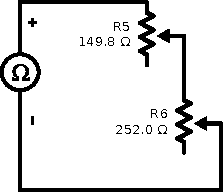
\includegraphics{Eletr1ResSerie.pdf} 
 \caption{Resistenza in serie} 
 \label{gr:02_graph_4.tex}
\end{figure}

\begin{figure}[width=0.7\textwidth]
 \centering 
 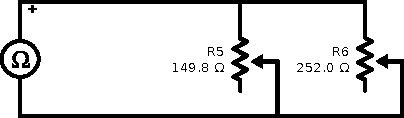
\includegraphics{Eletr1respar.pdf} 
 \caption{Resistenza in parallelo} 
 \label{gr:02_graph_4.tex}
\end{figure}

\begin{figure}[width=0.7\textwidth]
 \centering 
 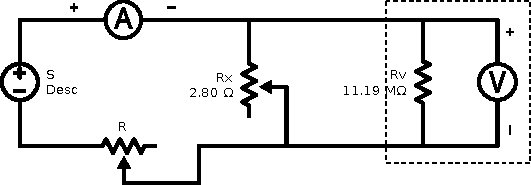
\includegraphics{Eletr1VoltAmpere.pdf} 
 \caption{Misura voltamperometrica} 
 \label{gr:02_graph_4.tex}
\end{figure}

% \begin{figure}[width=0.7\textwidth]
%  \centering 
%  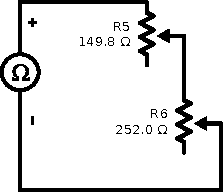
\includegraphics{Eletr1_ResSerie.pdf} 
%  \caption{Eletr1_ResSerie.pdf} 
%  \label{gr:02_graph_4.tex}
% \end{figure}

\begin{figure}[width=0.7\textwidth]
 \centering 
 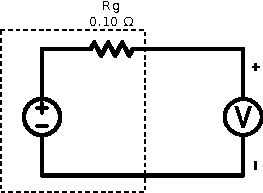
\includegraphics{Eletr1ResGeneratore.pdf} 
 \caption{Resistenza del generatore (I)} 
 \label{gr:02_graph_4.tex}
\end{figure}

\begin{figure}[width=0.7\textwidth]
 \centering 
 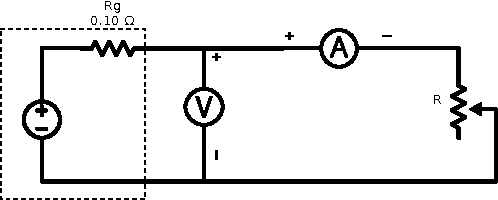
\includegraphics{Eletr1ResGeneratore2.pdf} 
 \caption{Resistenza del generatore (II)} 
 \label{gr:02_graph_4.tex}
\end{figure}

\begin{figure}[width=0.7\textwidth]
 \centering 
 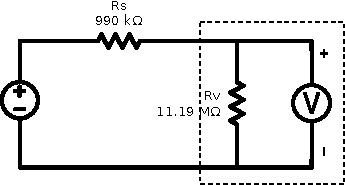
\includegraphics{Eletr1ResVoltmetro.pdf} 
 \caption{Resistenza voltmetro} 
 \label{gr:02_graph_4.tex}
\end{figure}

\begin{figure}[width=0.7\textwidth]
 \centering 
 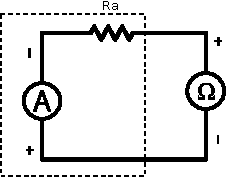
\includegraphics{Eletr1ResAmperometro.pdf} 
 \caption{Resistenza amperometro} 
 \label{gr:02_graph_4.tex}
\end{figure}
	%\subsection{Tabelle}
	%\begin{multicols}{2}
	%\input{./sezioni/pres_dati_tabelle.tex}
	%\end{multicols}
	%\clearpage
	%\subsection{Grafici}
	%\begin{grafico} \centering \input{../gnuplot/immagini/02_graph_1.tex} \caption{Grafico 02_graph_1.tex} \label{gr:02_graph_1.tex} \end{grafico}
\begin{grafico} \centering \input{../gnuplot/immagini/02_graph_3.tex} \caption{Grafico 02_graph_3.tex} \label{gr:02_graph_3.tex} \end{grafico}
\begin{grafico} \centering \input{../gnuplot/immagini/02_graph_4.tex} \caption{Grafico 02_graph_4.tex} \label{gr:02_graph_4.tex} \end{grafico}


%\clearpage
%\begin{multicols}{2}
\section{Analisi dei dati}
	
\subsection{Misure dirette di resistenze}
I valori riportati in tabella (valori in $\Omega$) sono quelli delle misure dirette delle resistenze, prese col multimetro FLUKE 111; il fondo scala \`e di $200mA$ per le correnti e di $600mV$ per le tensioni.

%tabella RES DIRETTE
\begin{tabella}
	\centering
	\begin{center}
\begin{tabulary}{\textwidth}{CCC}
\toprule
Posizione relativa della lente & Diametro fascio a $30 \cm$ & Diametro fascio a $130 \cm$ \\ \midrule
0.400 & 1.187 & 1.000 \\ \midrule
0.450 & 1.193 & 1.105 \\ \midrule
0.460 & 1.171 & 1.172 \\ \midrule
0.475 & 1.168 & 1.190 \\ \midrule
0.500 & 1.186 & 1.254 \\ \midrule
0.550 & 1.190 & 1.367 \\
\bottomrule
\end{tabulary}
\end{center}

	\caption{Misure dirette resistenze}
	\label{tab:01_tab_1.tex}
\end{tabella}


Per stimare gli errori si \`e usata la formula seguente:
%formula diretta
\[ \sigma_R =\sqrt{ \sigma_{\textrm{sist}}^2 + \sigma_{\textrm{stat}}^2}= 0.58 \sqrt{(R\cdot\Delta P)^2 + (n_{\textrm{digit}} \cdot \min(\textrm{FS}))^2}\]
Infatti gli errori legati alla misurazione sono dovuti sia a errori di scala ($ R= k _R \cdot R^{(r)} $), sia a errori casuali connessi al numero di digit. Per chiarezza di notazione, $\sigma^{(r)}$ \`e considerato errore statistico, mentre con $\sigma$ si intende l'errore totale.

Per quanto riguarda le resistenze $R_5$ e $R_6$ in serie, da una misurazione diretta effettuata col multimetro FLUKE 111 risulta che $R_{\textrm{S,sper}}= (402 \pm 2 )\Omega$. Col calcolo teorico, il valore di tale resistenza equivalente risulta invece $R_{\textrm{S, teor}}=(402 \pm 2 )\Omega$, dove per l'errore teorico \`e stato considerato che $R_{\textrm{S,teor}}=k\cdot(R_1^{(r)} + R_2^{(r)})$, infatti la k \`e costante in misurazioni successive, mantenendo il medesimo fondo scala. Con semplice propagazione degli errori risulta che 
\[\sigma_{R_{\textrm{S,teor}}}=\sqrt{(R_1+R_2)^2\cdot\sigma_k^2+\sigma_{R_1^{(r)}}^2+\sigma_{R_2^{(r)}}^2}\]
dove $\sigma_k$ \`e stata ricavata dall'errore percentuale fornito dal costruttore del multimetro e considerando k distribuito uniformemente:
\(\sigma_k=0.58 \cdot Err\%\). 
\`E stata calcolata la correlazione tra le due diverse stime della resistenza, considerando che la loro differenza dovrebbe essere nulla:
\[\Delta R = R_{\textrm{S,teor}} - {R_{\textrm{S,sper}}}\]
\[\lambda=\frac{\left|\Delta R - 0\right|}{\sigma_{\Delta R}}=0.5\]
con $\Delta R = k\cdot(R_{\textrm{S,sper}}^{(r)}-R_1^{(r)}-R_2^{(r)})$, da cui per propagazione si ricava che 
\[ \sigma_{\Delta R} = 
        \sqrt{ (\Delta R)^2 \sigma_k^2 + 3 \sigma_R^{(r) 2} }\]

Per il calcolo della resistenza equivalente a $R_5$ e $R_6$ in parallelo, il valore misurato con il multimetro FLUKE 111 \`e $R_{\textrm{P,sper}}= (94 \pm 2) \Omega$.
Il valore teorico \`e $R_{\textrm{P,teor}}=(94 \pm 0.5) \Omega$: considerando che $R_{\textrm{P,teor}}=k  \frac{R_5^{(r)} R_6^{(r)}}{R_5^{(r)} + R_6^{(r)}}$ e propagando, riutilizzando la medesima semplificazione sull'errore di scala, si ottiene 
\[\sigma_{\textrm{P,teor}}=\sqrt{\left(\frac{R_5 R_6}{R_5+R_6}\right)^2 \sigma_k^2 + \frac{R_5^4 + R_6^4}{(R_5 + R_6)^4}  \sigma_{R_{\textrm{P,teor}}^{(r)}}^2} .\]
Per il calcolo della compatibilit\`a, si sono utilizzate le medesime formule che per le resistenze in serie, opportunamente adattate (con la stessa convenzione per $\Delta R$):
\[\lambda=\frac{\left|\Delta R - 0\right|}{\sigma_{\Delta R}}=0.24\]
con $\Delta R = k\cdot(R_{\textrm{S,sper}}^{(r)}-R_1^{(r)}-R_2^{(r)})$, da cui per propagazione si ricava che 
\[ \sigma_{\Delta R} = 
        \sqrt{ (\Delta R)^2 \sigma_k^2 + 3 \sigma_R^{(r) 2} }\]


%%\[\lambda=
%%	\frac{ \left|(R_{\textrm{P,teor}}-R_{\textrm{P,sper}})-0 \right| } { \sigma_{R_{\textrm{P,teor}}}-\sigma_{R_{\textrm{P,sper}}}}=0.14.\] 

Nota bene: tutti i calcoli sono stati effettuati mantenendo un numero superiore di cifre significative, riducendone il numero solo in sede di presentazione dati.



 











\subsection{Misura voltamperometrica di una resistenza}
Per misurare una resistenza piccola \`e stato costruito un circuito come in figura (da aggiungersi). Una prima misura diretta \`e stata effettuata utilizzando il multimetro FLUKE 111, che \`e risultata $R_x=(3.0 \pm 0.1) \Omega$.
Costruito il circuito, si \`e variata la resistenza di carico e la potenza erogata dal generatore per indagare di quanto fosse la caduta di potenziale al variare della corrente che attraversa R. I dati ottenuti sono riportati in tabella. 

%tabella AMPERE-VOLT
\begin{tabella}
	\centering
	\begin{center}
\begin{tabulary}{\textwidth}{CC}
\toprule
i (mA) & V (mV) \\ \midrule
25.0 & 70.5 \\ \midrule
30.6 & 86.2 \\ \midrule
37.5 & 106.4 \\ \midrule
49.6 & 140.3 \\ \midrule
60.8 & 171.7 \\ \midrule
69.7 & 182.0 \\ \midrule
72.9 & 204.3 \\ \midrule
81.8 & 230.1 \\ \midrule
100.0 & 280.1 \\ \midrule
90.5 & 254.8 \\ 
\bottomrule
\end{tabulary}
\end{center}

	\caption{Misure caduta di potenziale}
	\label{tab:02_tab_1.tex}
\end{tabella}

In grafico sono riportate tali misure esprimendo V in funzione di I, sovrapposte a un fit lineare ottenuto col metodo della massima verosimiglianza.

\begin{grafico}
\centering
\begin{tikzpicture}[gnuplot]
%% generated with GNUPLOT 4.6p4 (Lua 5.1; terminal rev. 99, script rev. 100)
%% dom 29 mar 2015 11:48:38 CEST
\path (0.000,0.000) rectangle (12.500,8.750);
\gpcolor{color=gp lt color border}
\gpsetlinetype{gp lt border}
\gpsetlinewidth{1.00}
\draw[gp path] (1.504,0.985)--(1.684,0.985);
\draw[gp path] (11.947,0.985)--(11.767,0.985);
\node[gp node right] at (1.320,0.985) { 50};
\draw[gp path] (1.504,2.218)--(1.684,2.218);
\draw[gp path] (11.947,2.218)--(11.767,2.218);
\node[gp node right] at (1.320,2.218) { 100};
\draw[gp path] (1.504,3.450)--(1.684,3.450);
\draw[gp path] (11.947,3.450)--(11.767,3.450);
\node[gp node right] at (1.320,3.450) { 150};
\draw[gp path] (1.504,4.683)--(1.684,4.683);
\draw[gp path] (11.947,4.683)--(11.767,4.683);
\node[gp node right] at (1.320,4.683) { 200};
\draw[gp path] (1.504,5.916)--(1.684,5.916);
\draw[gp path] (11.947,5.916)--(11.767,5.916);
\node[gp node right] at (1.320,5.916) { 250};
\draw[gp path] (1.504,7.148)--(1.684,7.148);
\draw[gp path] (11.947,7.148)--(11.767,7.148);
\node[gp node right] at (1.320,7.148) { 300};
\draw[gp path] (1.504,8.381)--(1.684,8.381);
\draw[gp path] (11.947,8.381)--(11.767,8.381);
\node[gp node right] at (1.320,8.381) { 350};
\draw[gp path] (1.504,0.985)--(1.504,1.165);
\draw[gp path] (1.504,8.381)--(1.504,8.201);
\node[gp node center] at (1.504,0.677) { 20};
\draw[gp path] (3.593,0.985)--(3.593,1.165);
\draw[gp path] (3.593,8.381)--(3.593,8.201);
\node[gp node center] at (3.593,0.677) { 40};
\draw[gp path] (5.681,0.985)--(5.681,1.165);
\draw[gp path] (5.681,8.381)--(5.681,8.201);
\node[gp node center] at (5.681,0.677) { 60};
\draw[gp path] (7.770,0.985)--(7.770,1.165);
\draw[gp path] (7.770,8.381)--(7.770,8.201);
\node[gp node center] at (7.770,0.677) { 80};
\draw[gp path] (9.858,0.985)--(9.858,1.165);
\draw[gp path] (9.858,8.381)--(9.858,8.201);
\node[gp node center] at (9.858,0.677) { 100};
\draw[gp path] (11.947,0.985)--(11.947,1.165);
\draw[gp path] (11.947,8.381)--(11.947,8.201);
\node[gp node center] at (11.947,0.677) { 120};
\draw[gp path] (1.504,8.381)--(1.504,0.985)--(11.947,0.985)--(11.947,8.381)--cycle;
\node[gp node center,rotate=-270] at (0.246,4.683) {V (mV)};
\node[gp node center] at (6.725,0.215) {i (mA)};
\node[gp node right] at (10.479,1.627) {Retta interpolante};
\gpcolor{rgb color={1.000,0.004,0.004}}
\gpsetlinetype{gp lt plot 0}
\draw[gp path] (10.663,1.627)--(11.579,1.627);
\draw[gp path] (1.504,1.149)--(1.609,1.219)--(1.715,1.289)--(1.820,1.359)--(1.926,1.429)%
  --(2.031,1.499)--(2.137,1.568)--(2.242,1.638)--(2.348,1.708)--(2.453,1.778)--(2.559,1.848)%
  --(2.664,1.917)--(2.770,1.987)--(2.875,2.057)--(2.981,2.127)--(3.086,2.197)--(3.192,2.267)%
  --(3.297,2.336)--(3.403,2.406)--(3.508,2.476)--(3.614,2.546)--(3.719,2.616)--(3.825,2.686)%
  --(3.930,2.755)--(4.036,2.825)--(4.141,2.895)--(4.247,2.965)--(4.352,3.035)--(4.458,3.104)%
  --(4.563,3.174)--(4.669,3.244)--(4.774,3.314)--(4.880,3.384)--(4.985,3.454)--(5.090,3.523)%
  --(5.196,3.593)--(5.301,3.663)--(5.407,3.733)--(5.512,3.803)--(5.618,3.873)--(5.723,3.942)%
  --(5.829,4.012)--(5.934,4.082)--(6.040,4.152)--(6.145,4.222)--(6.251,4.291)--(6.356,4.361)%
  --(6.462,4.431)--(6.567,4.501)--(6.673,4.571)--(6.778,4.641)--(6.884,4.710)--(6.989,4.780)%
  --(7.095,4.850)--(7.200,4.920)--(7.306,4.990)--(7.411,5.059)--(7.517,5.129)--(7.622,5.199)%
  --(7.728,5.269)--(7.833,5.339)--(7.939,5.409)--(8.044,5.478)--(8.150,5.548)--(8.255,5.618)%
  --(8.361,5.688)--(8.466,5.758)--(8.571,5.828)--(8.677,5.897)--(8.782,5.967)--(8.888,6.037)%
  --(8.993,6.107)--(9.099,6.177)--(9.204,6.246)--(9.310,6.316)--(9.415,6.386)--(9.521,6.456)%
  --(9.626,6.526)--(9.732,6.596)--(9.837,6.665)--(9.943,6.735)--(10.048,6.805)--(10.154,6.875)%
  --(10.259,6.945)--(10.365,7.015)--(10.470,7.084)--(10.576,7.154)--(10.681,7.224)--(10.787,7.294)%
  --(10.892,7.364)--(10.998,7.433)--(11.103,7.503)--(11.209,7.573)--(11.314,7.643)--(11.420,7.713)%
  --(11.525,7.783)--(11.631,7.852)--(11.736,7.922)--(11.842,7.992)--(11.947,8.062);
\gpcolor{color=gp lt color border}
\node[gp node right] at (10.479,1.319) {Dati};
\gpcolor{rgb color={0.000,0.000,0.000}}
\gpsetpointsize{4.00}
\gppoint{gp mark 2}{(9.858,6.658)}
\gppoint{gp mark 2}{(7.028,4.789)}
\gppoint{gp mark 2}{(5.765,3.985)}
\gppoint{gp mark 2}{(3.332,2.375)}
\gppoint{gp mark 2}{(4.595,3.211)}
\gppoint{gp mark 2}{(8.866,6.034)}
\gppoint{gp mark 2}{(2.611,1.877)}
\gppoint{gp mark 2}{(2.026,1.490)}
\gppoint{gp mark 2}{(7.958,5.425)}
\gppoint{gp mark 2}{(6.172,4.239)}
\gppoint{gp mark 2}{(11.121,1.319)}
\gpcolor{color=gp lt color border}
\gpsetlinetype{gp lt border}
\draw[gp path] (1.504,8.381)--(1.504,0.985)--(11.947,0.985)--(11.947,8.381)--cycle;
%% coordinates of the plot area
\gpdefrectangularnode{gp plot 1}{\pgfpoint{1.504cm}{0.985cm}}{\pgfpoint{11.947cm}{8.381cm}}
\end{tikzpicture}
%% gnuplot variables

\caption{Fit lineare}
\label{fig:fitlin}
\end{grafico}

I coefficienti della retta interpolante $y=mx+c$ sono:
\[m = (2.809 \pm 0.004) \Omega \] 
\[c = (0.2 \pm 0.2) mV.\]
%Calcolando la covarianza tra $m$ e $c$ si ottiene 
%\[cov(m, c) = -0.000660084 V^4\] %UDM
Si \`e calcolata la correlazione 
\[\rho(m, c) = \frac{cov(m, c)}{\sigma_m \sigma_c}=-0.11\]
e l'errore a posteriori sulla caduta di tensione \`e di $\sigma_V=0.6V$.

A seguire il grafico dei residui: si \`e rappresentata la differenza tra il valore di tensione misurato e quello ricavato teoricamente dalla retta interpolante in corrispondenza del suo valore di corrente.

\begin{grafico}
\centering
\begin{tikzpicture}[gnuplot]
%% generated with GNUPLOT 4.6p4 (Lua 5.1; terminal rev. 99, script rev. 100)
%% dom 29 mar 2015 11:48:38 CEST
\path (0.000,0.000) rectangle (12.500,8.750);
\gpcolor{color=gp lt color border}
\gpsetlinetype{gp lt border}
\gpsetlinewidth{1.00}
\draw[gp path] (1.504,0.985)--(1.684,0.985);
\draw[gp path] (11.947,0.985)--(11.767,0.985);
\node[gp node right] at (1.320,0.985) {-1.5};
\draw[gp path] (1.504,2.218)--(1.684,2.218);
\draw[gp path] (11.947,2.218)--(11.767,2.218);
\node[gp node right] at (1.320,2.218) {-1};
\draw[gp path] (1.504,3.450)--(1.684,3.450);
\draw[gp path] (11.947,3.450)--(11.767,3.450);
\node[gp node right] at (1.320,3.450) {-0.5};
\draw[gp path] (1.504,4.683)--(1.684,4.683);
\draw[gp path] (11.947,4.683)--(11.767,4.683);
\node[gp node right] at (1.320,4.683) { 0};
\draw[gp path] (1.504,5.916)--(1.684,5.916);
\draw[gp path] (11.947,5.916)--(11.767,5.916);
\node[gp node right] at (1.320,5.916) { 0.5};
\draw[gp path] (1.504,7.148)--(1.684,7.148);
\draw[gp path] (11.947,7.148)--(11.767,7.148);
\node[gp node right] at (1.320,7.148) { 1};
\draw[gp path] (1.504,8.381)--(1.684,8.381);
\draw[gp path] (11.947,8.381)--(11.767,8.381);
\node[gp node right] at (1.320,8.381) { 1.5};
\draw[gp path] (1.504,0.985)--(1.504,1.165);
\draw[gp path] (1.504,8.381)--(1.504,8.201);
\node[gp node center] at (1.504,0.677) { 20};
\draw[gp path] (3.593,0.985)--(3.593,1.165);
\draw[gp path] (3.593,8.381)--(3.593,8.201);
\node[gp node center] at (3.593,0.677) { 40};
\draw[gp path] (5.681,0.985)--(5.681,1.165);
\draw[gp path] (5.681,8.381)--(5.681,8.201);
\node[gp node center] at (5.681,0.677) { 60};
\draw[gp path] (7.770,0.985)--(7.770,1.165);
\draw[gp path] (7.770,8.381)--(7.770,8.201);
\node[gp node center] at (7.770,0.677) { 80};
\draw[gp path] (9.858,0.985)--(9.858,1.165);
\draw[gp path] (9.858,8.381)--(9.858,8.201);
\node[gp node center] at (9.858,0.677) { 100};
\draw[gp path] (11.947,0.985)--(11.947,1.165);
\draw[gp path] (11.947,8.381)--(11.947,8.201);
\node[gp node center] at (11.947,0.677) { 120};
\draw[gp path] (1.504,8.381)--(1.504,0.985)--(11.947,0.985)--(11.947,8.381)--cycle;
\node[gp node center,rotate=-270] at (0.246,4.683) {V (mV)};
\node[gp node center] at (6.725,0.215) {i (mA)};
\node[gp node right] at (10.479,8.047) {Residui};
\gpcolor{rgb color={1.000,0.004,0.004}}
\gpsetlinetype{gp lt plot 0}
\draw[gp path] (10.663,8.047)--(11.579,8.047);
\draw[gp path] (10.663,8.137)--(10.663,7.957);
\draw[gp path] (11.579,8.137)--(11.579,7.957);
\draw[gp path] (9.858,1.537)--(9.858,4.317);
\draw[gp path] (9.768,1.537)--(9.948,1.537);
\draw[gp path] (9.768,4.317)--(9.948,4.317);
\draw[gp path] (7.028,1.531)--(7.028,4.311);
\draw[gp path] (6.938,1.531)--(7.118,1.531);
\draw[gp path] (6.938,4.311)--(7.118,4.311);
\draw[gp path] (5.765,4.596)--(5.765,7.375);
\draw[gp path] (5.675,4.596)--(5.855,4.596);
\draw[gp path] (5.675,7.375)--(5.855,7.375);
\draw[gp path] (4.783,4.328)--(4.783,7.108);
\draw[gp path] (4.693,4.328)--(4.873,4.328);
\draw[gp path] (4.693,7.108)--(4.873,7.108);
\draw[gp path] (3.332,4.273)--(3.332,7.053);
\draw[gp path] (3.242,4.273)--(3.422,4.273);
\draw[gp path] (3.242,7.053)--(3.422,7.053);
\draw[gp path] (4.595,4.413)--(4.595,7.193);
\draw[gp path] (4.505,4.413)--(4.685,4.413);
\draw[gp path] (4.505,7.193)--(4.685,7.193);
\draw[gp path] (8.866,4.671)--(8.866,7.450);
\draw[gp path] (8.776,4.671)--(8.956,4.671);
\draw[gp path] (8.776,7.450)--(8.956,7.450);
\draw[gp path] (2.611,2.052)--(2.611,4.832);
\draw[gp path] (2.521,2.052)--(2.701,2.052);
\draw[gp path] (2.521,4.832)--(2.701,4.832);
\draw[gp path] (2.026,1.961)--(2.026,4.740);
\draw[gp path] (1.936,1.961)--(2.116,1.961);
\draw[gp path] (1.936,4.740)--(2.116,4.740);
\draw[gp path] (7.958,3.767)--(7.958,6.547);
\draw[gp path] (7.868,3.767)--(8.048,3.767);
\draw[gp path] (7.868,6.547)--(8.048,6.547);
\draw[gp path] (6.172,3.097)--(6.172,5.876);
\draw[gp path] (6.082,3.097)--(6.262,3.097);
\draw[gp path] (6.082,5.876)--(6.262,5.876);
\gpsetpointsize{4.00}
\gppoint{gp mark 1}{(9.858,2.927)}
\gppoint{gp mark 1}{(7.028,2.921)}
\gppoint{gp mark 1}{(5.765,5.986)}
\gppoint{gp mark 1}{(4.783,5.718)}
\gppoint{gp mark 1}{(3.332,5.663)}
\gppoint{gp mark 1}{(4.595,5.803)}
\gppoint{gp mark 1}{(8.866,6.060)}
\gppoint{gp mark 1}{(2.611,3.442)}
\gppoint{gp mark 1}{(2.026,3.351)}
\gppoint{gp mark 1}{(7.958,5.157)}
\gppoint{gp mark 1}{(6.172,4.486)}
\gppoint{gp mark 1}{(11.121,8.047)}
\gpcolor{rgb color={0.000,0.000,0.000}}
\gpsetlinetype{gp lt plot 1}
\draw[gp path] (1.504,4.683)--(1.609,4.683)--(1.715,4.683)--(1.820,4.683)--(1.926,4.683)%
  --(2.031,4.683)--(2.137,4.683)--(2.242,4.683)--(2.348,4.683)--(2.453,4.683)--(2.559,4.683)%
  --(2.664,4.683)--(2.770,4.683)--(2.875,4.683)--(2.981,4.683)--(3.086,4.683)--(3.192,4.683)%
  --(3.297,4.683)--(3.403,4.683)--(3.508,4.683)--(3.614,4.683)--(3.719,4.683)--(3.825,4.683)%
  --(3.930,4.683)--(4.036,4.683)--(4.141,4.683)--(4.247,4.683)--(4.352,4.683)--(4.458,4.683)%
  --(4.563,4.683)--(4.669,4.683)--(4.774,4.683)--(4.880,4.683)--(4.985,4.683)--(5.090,4.683)%
  --(5.196,4.683)--(5.301,4.683)--(5.407,4.683)--(5.512,4.683)--(5.618,4.683)--(5.723,4.683)%
  --(5.829,4.683)--(5.934,4.683)--(6.040,4.683)--(6.145,4.683)--(6.251,4.683)--(6.356,4.683)%
  --(6.462,4.683)--(6.567,4.683)--(6.673,4.683)--(6.778,4.683)--(6.884,4.683)--(6.989,4.683)%
  --(7.095,4.683)--(7.200,4.683)--(7.306,4.683)--(7.411,4.683)--(7.517,4.683)--(7.622,4.683)%
  --(7.728,4.683)--(7.833,4.683)--(7.939,4.683)--(8.044,4.683)--(8.150,4.683)--(8.255,4.683)%
  --(8.361,4.683)--(8.466,4.683)--(8.571,4.683)--(8.677,4.683)--(8.782,4.683)--(8.888,4.683)%
  --(8.993,4.683)--(9.099,4.683)--(9.204,4.683)--(9.310,4.683)--(9.415,4.683)--(9.521,4.683)%
  --(9.626,4.683)--(9.732,4.683)--(9.837,4.683)--(9.943,4.683)--(10.048,4.683)--(10.154,4.683)%
  --(10.259,4.683)--(10.365,4.683)--(10.470,4.683)--(10.576,4.683)--(10.681,4.683)--(10.787,4.683)%
  --(10.892,4.683)--(10.998,4.683)--(11.103,4.683)--(11.209,4.683)--(11.314,4.683)--(11.420,4.683)%
  --(11.525,4.683)--(11.631,4.683)--(11.736,4.683)--(11.842,4.683)--(11.947,4.683);
\gpcolor{color=gp lt color border}
\gpsetlinetype{gp lt border}
\draw[gp path] (1.504,8.381)--(1.504,0.985)--(11.947,0.985)--(11.947,8.381)--cycle;
%% coordinates of the plot area
\gpdefrectangularnode{gp plot 1}{\pgfpoint{1.504cm}{0.985cm}}{\pgfpoint{11.947cm}{8.381cm}}
\end{tikzpicture}
%% gnuplot variables

\caption{Residui}
\label{fig:residui}
\end{grafico}

Una stima della resistenza \`e data dalla pendenza della retta interpolante. Tale retta ha un errore che \`e composizione di un errore sistematico e di uno statistico, infatti si pu\`o scrivere $m=\frac{k_V (V_2^{(r)}-V_1^{(r)})}{k_i (i_2^{(r)} - i_1^{(r)})}=\frac{k_V}{k_i}m^{(r)}$.
Da una propagazione risulta che l'errore su tale grandezza \`e $\sigma_m=\sqrt{\sigma_{\textrm{m,fit}}^2 + \sigma_{k_V}^2 m^2 + \sigma_{k_i}^2 m^2}$ con $\sigma_{\textrm{m,fit}}$ errore casuale ottenuto dall'interpolazione.
Risulta che l'incertezza sulla resistenza \`e quasi completamente data dall'errore sistematico. Il risultato finale \`e $R=(2.8 \pm 0.4) \Omega$; l'errore percentuale \`e del $13 \%$.

Si possono confrontare il risultato teorico e quello sperimentale con un calcolo di compatibilit\`a. Dato che sono state usate strumentazioni differenti per le due stime, se ne pu\`o applicare la definizione: 
$\lambda=\frac{|R_x - R|}{\sqrt{\sigma_{R_x}^2+\sigma_R^2}}=0.5$.
 











\subsection{Resistenze interne degli strumenti di misura}
Attraverso costruzioni di circuiti o misure dirette, si sono stimate le resistenze interne degli strumenti utilizzati.
Per la stima della resistenza interna del generatore si \`e costruito un circuito come in figura (da aggiungersi) e utilizzato il voltmetro AGILENT U1232A con l'amperometro BECKMAN T110B.
Dalle misure risulta che
\begin{align}
V_0 &=(5.01 \pm 0.01 )V \ \textrm{con}\  V_{\textrm{FS}}=6V \\
i   &=(124.9 \pm 0.5) mA \ \textrm{con}\  i_{\textrm{FS}}=200mA \\
V   &=(5.00 \pm 0.01) V \ \textrm{con}\  V_{\textrm{FS}}=6V.
\end{align}
Da uno studio del circuito si ricava la formula $R_G=\frac{V_0-V}{V}$.
Stimandone l'errore, per evitare problemi di correlazione si pu\`o scrivere $R_G=\frac{k_v (V_0^{(r)}- V^{(r)})}{i}$, da cui propagando: 
\[\sigma_{R_G}=\sqrt{R_G^2 \sigma_{k_V}^2 + \frac{(\sigma_{V^{(r)}}^2 + \sigma_{V_0^{(r)}}^2)}{i^2} + \frac{(V_0-V)^2}{i^4} \sigma_i^2},\] ricordando che per $\sigma_i$ si intende l'errore strumentale totale. Concludendo, $R_G= (0.10 \pm 0.16) \Omega$.

Un diverso circuito \`e stato costruito per stimare la resistenza interna dell'AGILENT U1232A utilizzato come voltmetro.
Una misurazione diretta di $R_V$ \`e stata ottenuta utilizzando come ohmetro il BECKMAN T110B: $R_{\textrm{V, sper}}=(11.2 \pm 0.1) M\Omega$, con fondo scala di $20 M\Omega$. 
Le misure prese a circuito chiuso sono: 
\begin{align}
R_S &= (0.990 \pm 0.005) M\Omega \ \textrm{con}\  R_{\textrm{FS}}=6 M\Omega \\
V_0 &= (5.01 \pm 0.01) V \ \textrm{con}\  V_{\textrm{FS}} = 6 V \\
V &= (4.60 \pm 0.01) V \ \textrm{con}\  V_{\textrm{FS}} = 6 V
\end{align}
Studiando il circuito, si pu\`o dimostrare che 
\[ R_{\textrm{V, teor}} = \frac{R_S V}{V_0 - V} . \]
Portando fuori dai valori il coefficiente $k_V$ e semplificandolo, si ha $R_{\textrm{V, teor}} = \frac{R_S V^{(r)}}{V_0^{(r)} - V^{(r)}}$ da cui, propagando, si ottiene \[\sigma_{R_{\textrm{V,teor}}} = \sqrt{\sigma_{R_S}^2 \left(\frac{V}{(V_0 - V)^2} \right)^2 + \sigma_{V_{(r)}}^2 \left(\frac{R_S V_0}{(V_0 - V)^2}\right)^2 + \sigma_{V_0^{(r) 2}} \left(\frac{R_S V}{(V_0 - V)^2}\right)^2}.\]
Risulta $R_{\textrm{V, teor}} = (11.19 \pm 0.08) M\Omega$.


Per misurare la resistenza interna del BECKMAN T110B, usato come amperometro, si \`e semplicemente effettuato un collegamento con il FLUKE 111 usato come ohmetro. I valori sono riportati in tabella.

%tabella RESISTENZE AMPEROMETRO
\begin{tabella}
	\centering
	\begin{center}
\begin{tabulary}{\textwidth}{CCCC}
\toprule
$I_{FS}$ & $R (\Omega)$ & $\sigma_R (\Omega)$ & $R_{FS} (\Omega)$ \\ \midrule
200 mA & 1002 & 5 & 6000 \\ \midrule
2 mA & 102.1 & 0.5 & 600 \\ \midrule
20 mA & 11.4 & 0.1 & 600 \\ \midrule
200 mA & 1.8 & 0.1 & 600 \\ \midrule
2 A & 1.2 & 0.1 & 600 \\ 
\bottomrule
\end{tabulary}
\end{center}

	\caption{Resistenze dell'amperometro BECKMAN}
	\label{tab:03_tab_1.tex}
\end{tabella}



\section{Appendice: calcolo degli errori}
	\label{sec:appendice}
Si riporta la formula usata per il calcolo dell'incertezza di una misura diretta $A \pm \sigma _A$:
\[  \sigma_A =\sqrt{ \sigma_{\textrm{sist}}^2 + \sigma_{\textrm{stat}}^2}= 0.58 \sqrt{\big(A\cdot\Delta P)^2 + (n_{\textrm{digit}} \cdot \min(\textrm{FS})\big)^2}\]
Infatti gli errori legati alla misurazione sono dovuti sia a errori di scala ($ A= k _A \cdot A^{(r)} $), sia a errori casuali connessi al numero di digit. Per chiarezza di notazione, $\sigma^{(r)}$ \`e considerato errore statistico, mentre con $\sigma$ si intende l'errore totale.

Inoltre, per stimare $\sigma _k$ si \`e utilizzato l'errore percentuale fornito dal costruttore del multimetro, considerando $k$ distribuito uniformemente:
\[\sigma _k = 0.58 \cdot \Delta _P \]

	
\section{Conclusioni}
	Tutti i valori misurati e calcolati sono coerenti e richiamano le aspettative fatte.
L'unica grandezza che rivela un parziale disaccordo tra i dati \`e la compatibilit\`a nel caso della misura voltamperometrica. Si evince comunque, dai grafici presentati, che la retta interpola sufficientemente bene i dati raccolti.

	
	%\end{multicols}
\newpage
\section{Codice}
} 	%Fine del grigio e di lsstyle

	\'E presentata qua la parte fondamentale del codice in c++ usato per i calcoli numerici. Inoltre è stato usato per i calcoli Mathematica.

\begin{lstlisting}[language=C++]
double interp_delta(int N, double * x, double * y)
{
	double delta=N*sumquad(N, x)-((sum(N, x))*(sum(N, x)));
	return delta;
}
double interp_a(int N, double * x, double * y)
{
	double a=(1/interp_delta(N, x, y))*((sumquad(N, x))*(sum(N, y))-(sum(N, x))*(sumprod (N, x, y)));
	return a;
}
double interp_b(int N, double * x, double * y)
{
	double b=(1/interp_delta(N, x, y))*(N*(sumprod(N, x, y))-((sum(N, x))*(sum(N, y))));
	return b;
}
double sigmay_post(int N, double * x, double * y)
{
	double sy=0;
	for (int i=0; i<N; i++){
		sy+=((interp_a(N, x, y))+((interp_b(N, x, y))*x[i])-(y[i]))*((interp_a(N, x, y))+((interp_b(N, x, y))*x[i])-(y[i]));
	}
	sy=sy/(N-2);
	sy=sqrt(sy);
	return sy;
}
double interp_sigmaa(int N, double * x, double * y)
{
	double sa=(sigmay_post(N, x, y))*sqrt((sumquad(N, x))/(interp_delta(N, x, y)));
	return sa;
}
double interp_sigmab(int N, double * x, double * y)
{
	double sb=(sigmay_post(N, x, y))*sqrt(N/(interp_delta(N, x, y)));
	return sb;
}
double cov_mq(int N, double * x, double * y)
{
	return (-(sum(N, x)*sigmay_post(N, x, y)*sigmay_post(N, x, y)/interp_delta(N, x, y)));
}
\end{lstlisting}

	
%\subsection{Esempio immagini}
%\begin{figure}[p]
% \centering
% \includegraphics[width=0.8\textwidth]{spazio1}
% \caption{Spazio!}
% \label{fig:spazio1}
%\end{figure}



\end{document}
